\chapter{Project realization}
\section{Introduction}
This chapter covers the implementation, testing and the deployment processes of
the Benchmarks dashboard project. To deal wit each of these processes, we will
introduce the technologies used and describe the way we used them. In
addition, we will presente the project planning.
\section{Developmnet environment}
\subsection{Devlopment machine characteristics}
The table  TODO presents the characteristics of the developmnet machine we used
during the project implementation.

\begin{center}
  \begin{tabular}{ | p{5cm}  | p{4cm}  | p{2cm} | }
    \hline

    \multicolumn{2}{|c|r|}{Characteristics } & Decription\\
    \hline

\multirow{3}{4em}{Processor} & Type & Intel® Core™ i7-3540M CPU \\ 
\multirow{3}{4em}{Processor} & Type & Intel® Core™ i7-3540M CPU \\ 
\multirow{3}{4em}{Processor} & Type & Intel® Core™ i7-3540M CPU \\ 

     99              & 99        \\ \hline
     99              & 99        \\ \hline

    \hline
  \end{tabular}
\end{center}


\section{Project management}
This section gives an overview of the project management process of the
Benchmarks Dashboard application. At first, we will start by introducing the
project team and then we will describe the tracking process of the different
implementation tasks.
\subsection{Project team}
The table TODO introduces the project team members and their roles.

\begin{center}
  \begin{tabular}{ | p{3cm}  | p{6cm} |}
    \hline

    Scrum role    & Person          \\ \hline

    Product owner & Oussama Elkaceh \\ \hline
    Scrum Master  & Wassel Msehli   \\ \hline
    Team members  & Chaker Benhamed \\ \hline

    \hline
  \end{tabular}
\end{center}

\subsection{Jira tool}
Predictix development teams use Jira for managing the projects. Jira is a
commercial software product developed by Atlassian. It is used for bug tracking,
issue tracking and project management. Jira allow prioritizing, assigning,
tracking, reporting and auditing issues. Indeed, it improves productivity by
cutting down on time wasted on tracking issues and coordination. In fact, it
keeps the team on track and allows the project manager to monitor the progress
on projects. Besides, it improves quality be ensuring that all tasks are
recorded down with all details and followed up until accomplishment. Moreover,
Jira is an extensible platform which means that it offers workflow customization
to match more the business process. TODO(Add link Atlassian, jira software
provider, www.atlassian.com.)


\section{Implementation}
\subsection{Implementation process}
This section descirbes the whole implementation process step by step TODO

\section{Deployment}
Hydra is a Nix-based continuous build system that constantly checks out code
sources of software projects from version management systems such as Mercurial,
to build, test and release them. The build tasks are described using Nix
expressions. This allows a Hydra build task to specify all the dependencies
needed to build or test a project.

In fact, the code of our application is, currently and constantly pushed in a
repository in BitBucket, which is a web-based hosting service for projects that
use either the Mercurial or Git revision control systems, such as GitHub. In
order to have our application ready to be deployed, we added a file called
default.nix to our project, that actually defines our project’s nix-expressions.
Afterwards, we created a project under Hydra, that we called \emph{Benchmarks
  Dashboard}. Thus, the \emph{Benchmarks Dashboard} project on Hydra, will be
pulling our code from our BitBucket repository along with the default.nix file
in order to perform the automated build and unit-tests.

The following are some screen shots about our Hydra project build. The figure
\hyperref[fig:hydra_configuration]{\ref{fig:hydra_configuration}}
represents the configuraton for our project. We can notice that the links to the
different project's dependecies are defined, such as our source code and the
nixpkgs repo which contains the definitions for all packages available through
the nix package manager.

\begin{figure}[h]
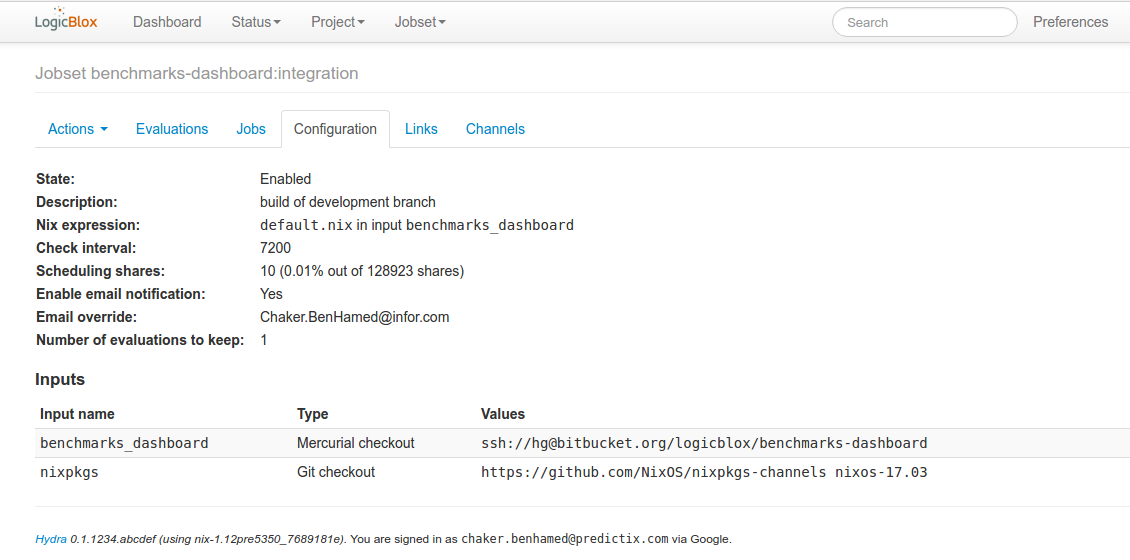
\includegraphics[width=17cm]{hydra_configuration}
\caption{Benchmarks Dashboard Hydra configuration screen}
\label{fig:hydra_configuration}
\end{figure}

The figure \hyperref[fig:hydra_eval]{\ref{fig:hydra_eval}} represents the Hydra
evaulation screen, where we can see the history if the build and whether there
are erros in the build or not.

\begin{figure}[h]
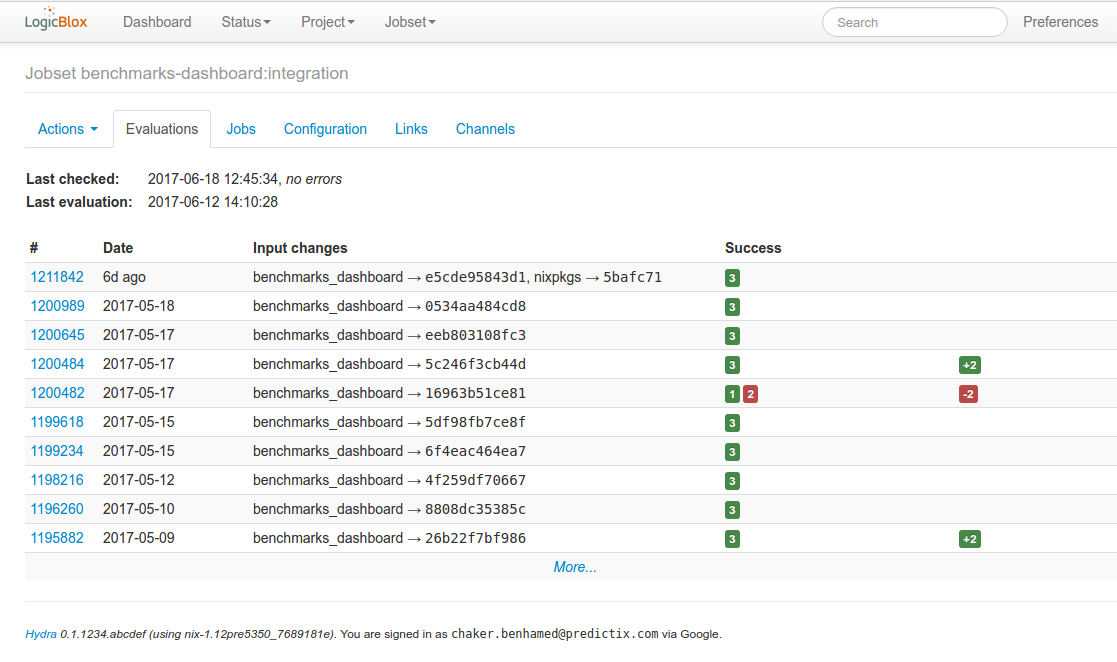
\includegraphics[width=17cm]{hydra_eval}
\caption{Benchmarks Dashboard Hydra configuration screen}
\label{fig:hydra_eval}
\end{figure}

In Hydra we can also run unit test and report various indicator about the
quality of the application. The figure
\hyperref[fig:coverage]{\ref{fig:coverage}} shows the covarge report of the test
of our application.

\begin{figure}[h]
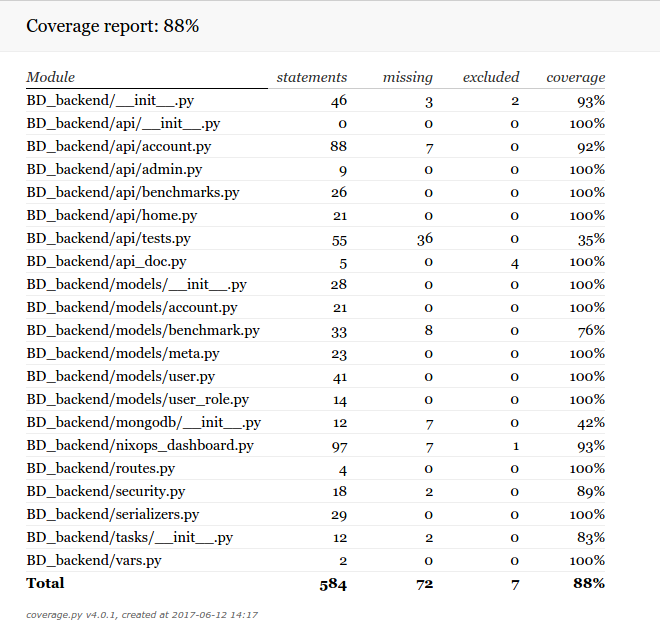
\includegraphics[width=17cm]{coverage}
\caption{Coverage report}
\label{fig:coverage}
\end{figure}

\section*{Conclusion}
TODO
